%% LyX 2.1.4 created this file.  For more info, see http://www.lyx.org/.
%% Do not edit unless you really know what you are doing.
\documentclass[english]{article}
\usepackage[T1]{fontenc}
\usepackage[latin9]{inputenc}
\usepackage{graphicx}

\makeatletter
%%%%%%%%%%%%%%%%%%%%%%%%%%%%%% User specified LaTeX commands.
%% ODER: format ==         = "\mathrel{==}"
%% ODER: format /=         = "\neq "
%
%
\makeatletter
\@ifundefined{lhs2tex.lhs2tex.sty.read}%
  {\@namedef{lhs2tex.lhs2tex.sty.read}{}%
   \newcommand\SkipToFmtEnd{}%
   \newcommand\EndFmtInput{}%
   \long\def\SkipToFmtEnd#1\EndFmtInput{}%
  }\SkipToFmtEnd

\newcommand\ReadOnlyOnce[1]{\@ifundefined{#1}{\@namedef{#1}{}}\SkipToFmtEnd}
\usepackage{amstext}
\usepackage{amssymb}
\usepackage{stmaryrd}
\DeclareFontFamily{OT1}{cmtex}{}
\DeclareFontShape{OT1}{cmtex}{m}{n}
  {<5><6><7><8>cmtex8
   <9>cmtex9
   <10><10.95><12><14.4><17.28><20.74><24.88>cmtex10}{}
\DeclareFontShape{OT1}{cmtex}{m}{it}
  {<-> ssub * cmtt/m/it}{}
\newcommand{\texfamily}{\fontfamily{cmtex}\selectfont}
\DeclareFontShape{OT1}{cmtt}{bx}{n}
  {<5><6><7><8>cmtt8
   <9>cmbtt9
   <10><10.95><12><14.4><17.28><20.74><24.88>cmbtt10}{}
\DeclareFontShape{OT1}{cmtex}{bx}{n}
  {<-> ssub * cmtt/bx/n}{}
\newcommand{\tex}[1]{\text{\texfamily#1}}	% NEU

\newcommand{\Sp}{\hskip.33334em\relax}


\newcommand{\Conid}[1]{\mathit{#1}}
\newcommand{\Varid}[1]{\mathit{#1}}
\newcommand{\anonymous}{\kern0.06em \vbox{\hrule\@width.5em}}
\newcommand{\plus}{\mathbin{+\!\!\!+}}
\newcommand{\bind}{\mathbin{>\!\!\!>\mkern-6.7mu=}}
\newcommand{\rbind}{\mathbin{=\mkern-6.7mu<\!\!\!<}}% suggested by Neil Mitchell
\newcommand{\sequ}{\mathbin{>\!\!\!>}}
\renewcommand{\leq}{\leqslant}
\renewcommand{\geq}{\geqslant}
\usepackage{polytable}

%mathindent has to be defined
\@ifundefined{mathindent}%
  {\newdimen\mathindent\mathindent\leftmargini}%
  {}%

\def\resethooks{%
  \global\let\SaveRestoreHook\empty
  \global\let\ColumnHook\empty}
\newcommand*{\savecolumns}[1][default]%
  {\g@addto@macro\SaveRestoreHook{\savecolumns[#1]}}
\newcommand*{\restorecolumns}[1][default]%
  {\g@addto@macro\SaveRestoreHook{\restorecolumns[#1]}}
\newcommand*{\aligncolumn}[2]%
  {\g@addto@macro\ColumnHook{\column{#1}{#2}}}

\resethooks

\newcommand{\onelinecommentchars}{\quad-{}- }
\newcommand{\commentbeginchars}{\enskip\{-}
\newcommand{\commentendchars}{-\}\enskip}

\newcommand{\visiblecomments}{%
  \let\onelinecomment=\onelinecommentchars
  \let\commentbegin=\commentbeginchars
  \let\commentend=\commentendchars}

\newcommand{\invisiblecomments}{%
  \let\onelinecomment=\empty
  \let\commentbegin=\empty
  \let\commentend=\empty}

\visiblecomments

\newlength{\blanklineskip}
\setlength{\blanklineskip}{0.66084ex}

\newcommand{\hsindent}[1]{\quad}% default is fixed indentation
\let\hspre\empty
\let\hspost\empty
\newcommand{\NB}{\textbf{NB}}
\newcommand{\Todo}[1]{$\langle$\textbf{To do:}~#1$\rangle$}

\EndFmtInput
\makeatother
%
%
%
%
%
%
% This package provides two environments suitable to take the place
% of hscode, called "plainhscode" and "arrayhscode". 
%
% The plain environment surrounds each code block by vertical space,
% and it uses \abovedisplayskip and \belowdisplayskip to get spacing
% similar to formulas. Note that if these dimensions are changed,
% the spacing around displayed math formulas changes as well.
% All code is indented using \leftskip.
%
% Changed 19.08.2004 to reflect changes in colorcode. Should work with
% CodeGroup.sty.
%
\ReadOnlyOnce{polycode.fmt}%
\makeatletter

\newcommand{\hsnewpar}[1]%
  {{\parskip=0pt\parindent=0pt\par\vskip #1\noindent}}

% can be used, for instance, to redefine the code size, by setting the
% command to \small or something alike
\newcommand{\hscodestyle}{}

% The command \sethscode can be used to switch the code formatting
% behaviour by mapping the hscode environment in the subst directive
% to a new LaTeX environment.

\newcommand{\sethscode}[1]%
  {\expandafter\let\expandafter\hscode\csname #1\endcsname
   \expandafter\let\expandafter\endhscode\csname end#1\endcsname}

% "compatibility" mode restores the non-polycode.fmt layout.

\newenvironment{compathscode}%
  {\par\noindent
   \advance\leftskip\mathindent
   \hscodestyle
   \let\\=\@normalcr
   \let\hspre\(\let\hspost\)%
   \pboxed}%
  {\endpboxed\)%
   \par\noindent
   \ignorespacesafterend}

\newcommand{\compaths}{\sethscode{compathscode}}

% "plain" mode is the proposed default.
% It should now work with \centering.
% This required some changes. The old version
% is still available for reference as oldplainhscode.

\newenvironment{plainhscode}%
  {\hsnewpar\abovedisplayskip
   \advance\leftskip\mathindent
   \hscodestyle
   \let\hspre\(\let\hspost\)%
   \pboxed}%
  {\endpboxed%
   \hsnewpar\belowdisplayskip
   \ignorespacesafterend}

\newenvironment{oldplainhscode}%
  {\hsnewpar\abovedisplayskip
   \advance\leftskip\mathindent
   \hscodestyle
   \let\\=\@normalcr
   \(\pboxed}%
  {\endpboxed\)%
   \hsnewpar\belowdisplayskip
   \ignorespacesafterend}

% Here, we make plainhscode the default environment.

\newcommand{\plainhs}{\sethscode{plainhscode}}
\newcommand{\oldplainhs}{\sethscode{oldplainhscode}}
\plainhs

% The arrayhscode is like plain, but makes use of polytable's
% parray environment which disallows page breaks in code blocks.

\newenvironment{arrayhscode}%
  {\hsnewpar\abovedisplayskip
   \advance\leftskip\mathindent
   \hscodestyle
   \let\\=\@normalcr
   \(\parray}%
  {\endparray\)%
   \hsnewpar\belowdisplayskip
   \ignorespacesafterend}

\newcommand{\arrayhs}{\sethscode{arrayhscode}}

% The mathhscode environment also makes use of polytable's parray 
% environment. It is supposed to be used only inside math mode 
% (I used it to typeset the type rules in my thesis).

\newenvironment{mathhscode}%
  {\parray}{\endparray}

\newcommand{\mathhs}{\sethscode{mathhscode}}

% texths is similar to mathhs, but works in text mode.

\newenvironment{texthscode}%
  {\(\parray}{\endparray\)}

\newcommand{\texths}{\sethscode{texthscode}}

% The framed environment places code in a framed box.

\def\codeframewidth{\arrayrulewidth}
\RequirePackage{calc}

\newenvironment{framedhscode}%
  {\parskip=\abovedisplayskip\par\noindent
   \hscodestyle
   \arrayrulewidth=\codeframewidth
   \tabular{@{}|p{\linewidth-2\arraycolsep-2\arrayrulewidth-2pt}|@{}}%
   \hline\framedhslinecorrect\\{-1.5ex}%
   \let\endoflinesave=\\
   \let\\=\@normalcr
   \(\pboxed}%
  {\endpboxed\)%
   \framedhslinecorrect\endoflinesave{.5ex}\hline
   \endtabular
   \parskip=\belowdisplayskip\par\noindent
   \ignorespacesafterend}

\newcommand{\framedhslinecorrect}[2]%
  {#1[#2]}

\newcommand{\framedhs}{\sethscode{framedhscode}}

% The inlinehscode environment is an experimental environment
% that can be used to typeset displayed code inline.

\newenvironment{inlinehscode}%
  {\(\def\column##1##2{}%
   \let\>\undefined\let\<\undefined\let\\\undefined
   \newcommand\>[1][]{}\newcommand\<[1][]{}\newcommand\\[1][]{}%
   \def\fromto##1##2##3{##3}%
   \def\nextline{}}{\) }%

\newcommand{\inlinehs}{\sethscode{inlinehscode}}

% The joincode environment is a separate environment that
% can be used to surround and thereby connect multiple code
% blocks.

\newenvironment{joincode}%
  {\let\orighscode=\hscode
   \let\origendhscode=\endhscode
   \def\endhscode{\def\hscode{\endgroup\def\@currenvir{hscode}\\}\begingroup}
   %\let\SaveRestoreHook=\empty
   %\let\ColumnHook=\empty
   %\let\resethooks=\empty
   \orighscode\def\hscode{\endgroup\def\@currenvir{hscode}}}%
  {\origendhscode
   \global\let\hscode=\orighscode
   \global\let\endhscode=\origendhscode}%

\makeatother
\EndFmtInput
%

\makeatother

\usepackage{babel}
\begin{document}

\author{David Spies}


\title{A list-based Sieve of Eratosthenes}

\maketitle
Contrary to O'Neill's claims in \textquotedbl{}The Genuine Sieve of
Eratosthenes\textquotedbl{}, it's possible to build an efficient Sieve
of Eratosthenes using only lists. This document is literate Haskell.
It compiles and runs on GHC 8.2.2. To compile it we'll need a main
method. Let's print out the first 30 primes:

\begin{hscode}\SaveRestoreHook
\column{B}{@{}>{\hspre}l<{\hspost}@{}}%
\column{E}{@{}>{\hspre}l<{\hspost}@{}}%
\>[B]{}\Varid{main}\mathbin{::}\Conid{IO}\;(){}\<[E]%
\\
\>[B]{}\Varid{main}\mathrel{=}\Varid{print}\;(\Varid{take}\;\mathrm{30}\;\Varid{primes}){}\<[E]%
\ColumnHook
\end{hscode}\resethooks

All lists used in this document are infinite and sorted. All lists
of lists are sorted on their heads. First, lets define a merge function
(for infinite sorted lists).

\begin{hscode}\SaveRestoreHook
\column{B}{@{}>{\hspre}l<{\hspost}@{}}%
\column{3}{@{}>{\hspre}l<{\hspost}@{}}%
\column{E}{@{}>{\hspre}l<{\hspost}@{}}%
\>[B]{}\Varid{merge}\mathbin{::}\Conid{Ord}\;\Varid{a}\Rightarrow [\mskip1.5mu \Varid{a}\mskip1.5mu]\to [\mskip1.5mu \Varid{a}\mskip1.5mu]\to [\mskip1.5mu \Varid{a}\mskip1.5mu]{}\<[E]%
\\
\>[B]{}\Varid{merge}\;(\Varid{x}\mathbin{:}\Varid{xs})\;(\Varid{y}\mathbin{:}\Varid{ys}){}\<[E]%
\\
\>[B]{}\hsindent{3}{}\<[3]%
\>[3]{}\mid \Varid{y}\mathbin{<}\Varid{x}\mathrel{=}\Varid{y}\mathbin{:}\Varid{merge}\;(\Varid{x}\mathbin{:}\Varid{xs})\;\Varid{ys}{}\<[E]%
\\
\>[B]{}\hsindent{3}{}\<[3]%
\>[3]{}\mid \Varid{otherwise}\mathrel{=}\Varid{x}\mathbin{:}\Varid{merge}\;\Varid{xs}\;(\Varid{y}\mathbin{:}\Varid{ys}){}\<[E]%
\ColumnHook
\end{hscode}\resethooks

This takes two sorted lists and merges them into a single sorted list.
Note that evaluating the head of the result triggers the evaluation
of both arguments' heads. We'll need a version that takes the head
of the left argument and puts that as the head of the result before
ever evaluating the right argument. Then we'll be careful to call
it only where we know the head of the right list is at least as large
as the head of the left. 

\begin{hscode}\SaveRestoreHook
\column{B}{@{}>{\hspre}l<{\hspost}@{}}%
\column{E}{@{}>{\hspre}l<{\hspost}@{}}%
\>[B]{}\Varid{fmerge}\mathbin{::}\Conid{Ord}\;\Varid{a}\Rightarrow [\mskip1.5mu \Varid{a}\mskip1.5mu]\to [\mskip1.5mu \Varid{a}\mskip1.5mu]\to [\mskip1.5mu \Varid{a}\mskip1.5mu]{}\<[E]%
\\
\>[B]{}\Varid{fmerge}\;(\Varid{x}\mathbin{:}\Varid{xs})\;\Varid{ys}\mathrel{=}\Varid{x}\mathbin{:}\Varid{merge}\;\Varid{xs}\;\Varid{ys}{}\<[E]%
\ColumnHook
\end{hscode}\resethooks

With this in hand, we could define a function which lists all numbers
whose only prime factors are 2 and 3 as follows: 

\begin{hscode}\SaveRestoreHook
\column{B}{@{}>{\hspre}l<{\hspost}@{}}%
\column{E}{@{}>{\hspre}l<{\hspost}@{}}%
\>[B]{}\Varid{twosThreesOnly}\mathbin{::}[\mskip1.5mu \Conid{Integer}\mskip1.5mu]{}\<[E]%
\\
\>[B]{}\Varid{twosThreesOnly}\mathrel{=}\Varid{fmerge}\;(\Varid{iterate}\;(\mathrm{2}\mathbin{*})\;\mathrm{1})\;[\mskip1.5mu \mathrm{3}\mathbin{*}\Varid{x}\mid \Varid{x}\leftarrow \Varid{twosThreesOnly}\mskip1.5mu]{}\<[E]%
\ColumnHook
\end{hscode}\resethooks

We can also use\inputencoding{latin1}{ \texttt{fmerge}}\inputencoding{latin9}
to merge an infinite list of sorted lists together if we know the
heads of the lists are already sorted.

\begin{hscode}\SaveRestoreHook
\column{B}{@{}>{\hspre}l<{\hspost}@{}}%
\column{E}{@{}>{\hspre}l<{\hspost}@{}}%
\>[B]{}\Varid{fmergeAllNaive}\mathbin{::}\Conid{Ord}\;\Varid{a}\Rightarrow [\mskip1.5mu [\mskip1.5mu \Varid{a}\mskip1.5mu]\mskip1.5mu]\to [\mskip1.5mu \Varid{a}\mskip1.5mu]{}\<[E]%
\\
\>[B]{}\Varid{fmergeAllNaive}\;(\Varid{x}\mathbin{:}\Varid{xs})\mathrel{=}\Varid{fmerge}\;\Varid{x}\;(\Varid{fmergeAllNaive}\;\Varid{xs}){}\<[E]%
\ColumnHook
\end{hscode}\resethooks

This works and uses an impressively small amount of code, but isn't
very performant. In the worst case, evaluating the $k$th element
can require $O\left(k\right)$ running time. To see why this is, let's
look at what structure results from evaluating \texttt{fmergeAllNaive}
on a list. Suppose we have the list

\begin{hscode}\SaveRestoreHook
\column{B}{@{}>{\hspre}l<{\hspost}@{}}%
\column{E}{@{}>{\hspre}l<{\hspost}@{}}%
\>[B]{}\Varid{xs}\mathrel{=}\Varid{x1}\mathbin{:}\Varid{x2}\mathbin{:}\Varid{x3}\mathbin{:}\Varid{x4}\mathbin{:}\mathbin{...}{}\<[E]%
\ColumnHook
\end{hscode}\resethooks

When we call \texttt{fmergeAllNaive xs}, the resulting structure looks
something like Figure \ref{fig:fmergeallnaive}.

\begin{figure}


\caption{\label{fig:fmergeallnaive}Structure of \texttt{fmergeAllNaive}}


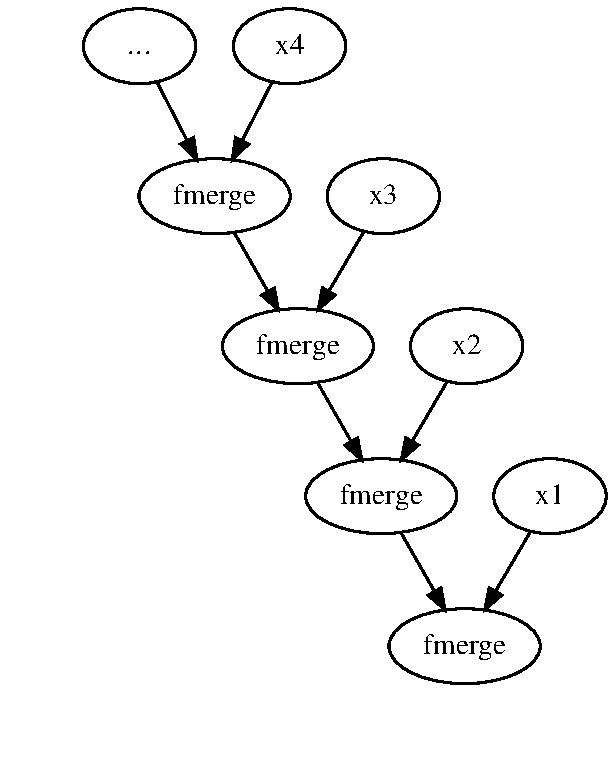
\includegraphics[height=0.3\textheight]{images/fig1}

\end{figure}


If an element belongs to list $x_{k}$, then to ``bubble up'' to the
top of our evaluation structure, it must be compared against the first
element of $x_{k-1}$, followed by the first element of $x_{k-2}$
etc. until finally being compared against $x_{1}$.

To rectify this, let's first create a helper function for efficiently
merging a list prefix of length-$k$ (where $k>0$). The \texttt{fmergePrefix}
function returns both the merged prefix and the unmerged remainder.
As before, we assume the heads of the lists are themselves already
sorted.

\begin{hscode}\SaveRestoreHook
\column{B}{@{}>{\hspre}l<{\hspost}@{}}%
\column{3}{@{}>{\hspre}l<{\hspost}@{}}%
\column{5}{@{}>{\hspre}l<{\hspost}@{}}%
\column{E}{@{}>{\hspre}l<{\hspost}@{}}%
\>[B]{}\Varid{fmergePrefix}\mathbin{::}\Conid{Ord}\;\Varid{a}\Rightarrow \Conid{Int}\to [\mskip1.5mu [\mskip1.5mu \Varid{a}\mskip1.5mu]\mskip1.5mu]\to ([\mskip1.5mu \Varid{a}\mskip1.5mu],[\mskip1.5mu [\mskip1.5mu \Varid{a}\mskip1.5mu]\mskip1.5mu]){}\<[E]%
\\
\>[B]{}\Varid{fmergePrefix}\;\mathrm{1}\;(\Varid{x}\mathbin{:}\Varid{xs})\mathrel{=}(\Varid{x},\Varid{xs}){}\<[E]%
\\
\>[B]{}\Varid{fmergePrefix}\;\Varid{k}\;\Varid{xs}\mathrel{=}(\Varid{fmerge}\;\Varid{y}\;\Varid{z},\Varid{zs}){}\<[E]%
\\
\>[B]{}\hsindent{3}{}\<[3]%
\>[3]{}\mathbf{where}{}\<[E]%
\\
\>[3]{}\hsindent{2}{}\<[5]%
\>[5]{}(\Varid{y},\Varid{ys})\mathrel{=}\Varid{fmergePrefix}\;(\Varid{k}\mathbin{\Varid{`quot`}}\mathrm{2})\;\Varid{xs}{}\<[E]%
\\
\>[3]{}\hsindent{2}{}\<[5]%
\>[5]{}(\Varid{z},\Varid{zs})\mathrel{=}\Varid{fmergePrefix}\;((\Varid{k}\mathbin{+}\mathrm{1})\mathbin{\Varid{`quot`}}\mathrm{2})\;\Varid{ys}{}\<[E]%
\ColumnHook
\end{hscode}\resethooks

This should look familliarly like a standard merge-sort, except that
we're using \texttt{fmerge} rather than \texttt{merge} and all our
lists are infinite.

Notice that evaluating the first $n$ elements of the resulting merged
prefix requires at most $O\left(n\log k\right)$ steps as any element
needs to be compared with at most $\log_{2}k$ others to bubble to
the top. Now here's a more efficient \texttt{fmergeAll} implementation
which makes use of \texttt{fmergePrefix}. 

\begin{hscode}\SaveRestoreHook
\column{B}{@{}>{\hspre}l<{\hspost}@{}}%
\column{3}{@{}>{\hspre}l<{\hspost}@{}}%
\column{5}{@{}>{\hspre}l<{\hspost}@{}}%
\column{E}{@{}>{\hspre}l<{\hspost}@{}}%
\>[B]{}\Varid{fmergeAll}\mathbin{::}\Conid{Ord}\;\Varid{a}\Rightarrow [\mskip1.5mu [\mskip1.5mu \Varid{a}\mskip1.5mu]\mskip1.5mu]\to [\mskip1.5mu \Varid{a}\mskip1.5mu]{}\<[E]%
\\
\>[B]{}\Varid{fmergeAll}\mathrel{=}\Varid{go}\;\mathrm{1}{}\<[E]%
\\
\>[B]{}\hsindent{3}{}\<[3]%
\>[3]{}\mathbf{where}{}\<[E]%
\\
\>[3]{}\hsindent{2}{}\<[5]%
\>[5]{}\Varid{go}\;\Varid{k}\;\Varid{xs}\mathrel{=}\mathbf{let}\;(\Varid{ys},\Varid{zs})\mathrel{=}\Varid{fmergePrefix}\;\Varid{k}\;\Varid{xs}\;\mathbf{in}\;\Varid{fmerge}\;\Varid{ys}\;(\Varid{go}\;(\Varid{k}\mathbin{*}\mathrm{2})\;\Varid{zs}){}\<[E]%
\ColumnHook
\end{hscode}\resethooks

\texttt{fmergeAll} is quite similar to \texttt{fmergeAllNaive} except
that instead of merging lists together one at a time, we merge them
in batches of exponentially growing size. Each batch is efficiently
merged using fmergePrefix. A consequence is that any element from
the $k^{\mbox{th}}$ list needs to be compared with at most $O\left(\log k\right)$
elements to bubble to the top of the resulting structure of thunks
(see Figure \ref{fig:fmergeall}). 

\begin{figure}


\caption{\label{fig:fmergeall}Structure of \texttt{fmergeAll}}


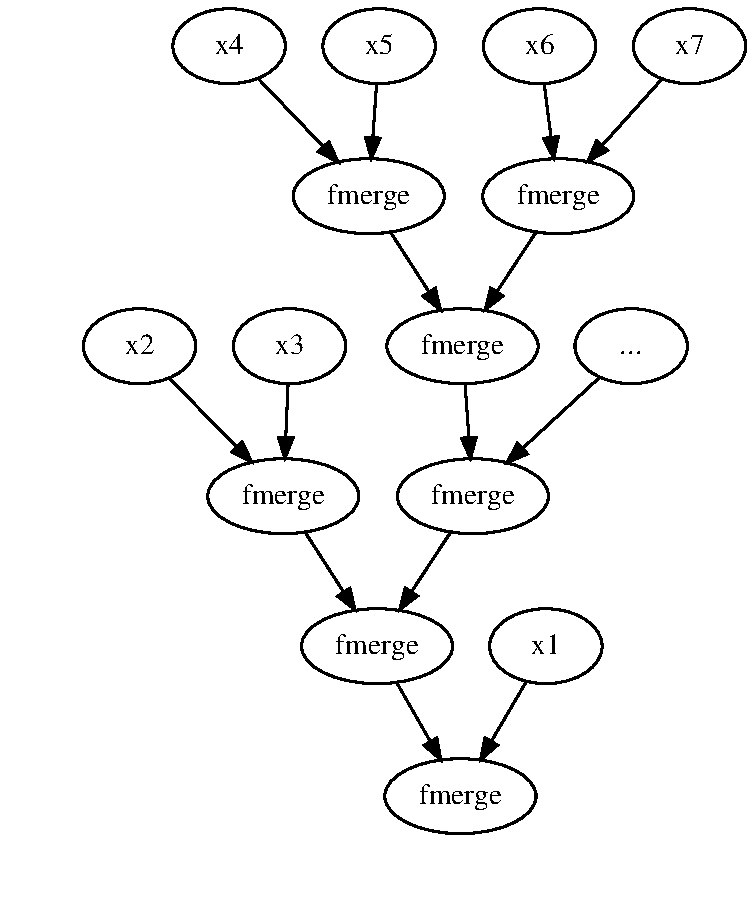
\includegraphics[height=0.3\textheight]{images/fig2}

\end{figure}


In addition to merging lists, it will also be useful to \emph{exclude}
elements from a list. The implementation is straightforward. 

\begin{hscode}\SaveRestoreHook
\column{B}{@{}>{\hspre}l<{\hspost}@{}}%
\column{3}{@{}>{\hspre}l<{\hspost}@{}}%
\column{E}{@{}>{\hspre}l<{\hspost}@{}}%
\>[B]{}\Varid{excluding}\mathbin{::}\Conid{Ord}\;\Varid{a}\Rightarrow [\mskip1.5mu \Varid{a}\mskip1.5mu]\to [\mskip1.5mu \Varid{a}\mskip1.5mu]\to [\mskip1.5mu \Varid{a}\mskip1.5mu]{}\<[E]%
\\
\>[B]{}(\Varid{x}\mathbin{:}\Varid{xs})\mathbin{`\Varid{excluding}`}(\Varid{y}\mathbin{:}\Varid{ys})\mathrel{=}\mathbf{case}\;\Varid{compare}\;\Varid{x}\;\Varid{y}\;\mathbf{of}{}\<[E]%
\\
\>[B]{}\hsindent{3}{}\<[3]%
\>[3]{}\Conid{LT}\to \Varid{x}\mathbin{:}(\Varid{xs}\mathbin{`\Varid{excluding}`}(\Varid{y}\mathbin{:}\Varid{ys})){}\<[E]%
\\
\>[B]{}\hsindent{3}{}\<[3]%
\>[3]{}\Conid{EQ}\to \Varid{xs}\mathbin{`\Varid{excluding}`}\Varid{ys}{}\<[E]%
\\
\>[B]{}\hsindent{3}{}\<[3]%
\>[3]{}\Conid{GT}\to (\Varid{x}\mathbin{:}\Varid{xs})\mathbin{`\Varid{excluding}`}\Varid{ys}{}\<[E]%
\ColumnHook
\end{hscode}\resethooks

With this in hand, we can mutually recursively define two lists: \texttt{primes}
and \texttt{composites} which respectively are lists of all the prime
and composite integers. The composites are the merged multiples of
the prime numbers. Note that if we start from the square of each prime,
then any composite number $n$ will occur once in the composites list
for each of its prime factors $p\le\sqrt{n}$ (every composite number
must have such a factor). The primes are then just the list of all
numbers larger than $1$ excluding the composites. To avoid unbounded
recursion, the number $2$ must be explicitly given as a prime. 

\begin{hscode}\SaveRestoreHook
\column{B}{@{}>{\hspre}l<{\hspost}@{}}%
\column{E}{@{}>{\hspre}l<{\hspost}@{}}%
\>[B]{}\Varid{primes}\mathbin{::}[\mskip1.5mu \Conid{Integer}\mskip1.5mu]{}\<[E]%
\\
\>[B]{}\Varid{primes}\mathrel{=}\mathrm{2}\mathbin{:}([\mskip1.5mu \mathrm{3}\mathinner{\ldotp\ldotp}\mskip1.5mu]\mathbin{`\Varid{excluding}`}\Varid{composites}){}\<[E]%
\\[\blanklineskip]%
\>[B]{}\Varid{composites}\mathbin{::}[\mskip1.5mu \Conid{Integer}\mskip1.5mu]{}\<[E]%
\\
\>[B]{}\Varid{composites}\mathrel{=}\Varid{fmergeAll}\;[\mskip1.5mu [\mskip1.5mu \Varid{p}\mathbin{*}\Varid{p},\Varid{p}\mathbin{*}(\Varid{p}\mathbin{+}\mathrm{1})\mathinner{\ldotp\ldotp}\mskip1.5mu]\mid \Varid{p}\leftarrow \Varid{primes}\mskip1.5mu]{}\<[E]%
\ColumnHook
\end{hscode}\resethooks

And that's it. \texttt{primes} is an efficient list of all the prime
numbers.
\end{document}
